\section{Fotoeffekt}


\begin{enumerate}

\item Fotoeffekt qanday hodisa?
\begin{enumerate}[label=\Alph*)]
\item Yorug‘likning bir muhitdan ikkinchi muhitga o‘tganida sinish hodisasi.
\item Jismlarning issiqdan kengayishi.
\item Yorug‘likning turli sirtlardan qaytish hodisasi.
\item Yorug‘lik ta’sirida moddalardan elektronning uzilib chiqishi.
\end{enumerate}

\setcounter{enumi}{1}
\item Metall sirtiga tushayotgan yorug‘lik chastotasi uchun qanday shart bajarilsa, fotoeffekt hodisasi kuzatiladi?
\begin{enumerate}[label=\Alph*)]
\item $\nu = A/h$.
\item $\nu > E_k/h$.
\item $\nu > (A+E_k)/h$.
\item $\nu \ge A/h$.
\end{enumerate}

\item Quyidagi parametrlarning qaysilari fotoeffektning qizil chegarasini aniqlaydi?
1) yorug‘lik chastotasi; 2) katodning chiqish ishi; 3) katod yuzi; 4) yorug‘lik intensivligi.
\begin{enumerate}[label=\Alph*)]
\item 1 va 4.
\item 3 va 4.
\item faqat 2.
\item 1 va 2.
\end{enumerate}

\item Fotoeffektning qizil chegarasini aniqlovchi formulani ko‘rsating.
\begin{enumerate}[label=\Alph*)]
\item $\lambda = cA/h$.
\item $\lambda = hc/A$.
\item $\lambda = Ah/c$.
\item $\lambda = A/ch$.
\end{enumerate}

\setcounter{enumi}{4}
\item Fotoeffekt uchun Eynshteyn tenglamasidagi $mv^2/2$ had nimani bildiradi?
\begin{enumerate}[label=\Alph*)]
\item atomdagi elektron energiyasini.
\item tushuvchi foton energiyasini.
\item atomdan urib chiqarilgan elektron kinetik energiyasini.
\item moddadagi atomlarning kinetik energiyasini.
\end{enumerate}

\item Elektronlarning chiqish ishi 3 eV bo‘lgan metall sirtiga 2 eV energiyaga ega bo‘lgan foton tushganda, fotoelektronlarning maksimal kinetik energiyasi nimaga teng bo‘ladi (eV)?
\begin{enumerate}[label=\Alph*)]
\item bu holda fotoeffekt yuz bermaydi.
\item 1.
\item 2.
\item 3.
\end{enumerate}

\item Elektronning chiqish ishi 3 eV bo‘lgan metallga energiyasi 5 eV bo‘lgan foton tushganda, elektronlarning maksimal kinetik energiyasi qanday (eV) bo‘ladi?
\begin{enumerate}[label=\Alph*)]
\item 0,6.
\item 2.
\item 3.
\item 5.
\end{enumerate}

\item Volfram chastotasi $1,933\cdot 10^{15}$ Hz bo‘lgan nurlar bilan yoritilmoqda, elektronlar uchun volframdan chiqish ishi 4,5 eV ga teng. Fotoelektronlarning maksimal kinetik energiyasini toping (eV).
\begin{enumerate}[label=\Alph*)]
\item 6,6.
\item 2,1.
\item 3,5.
\item 4.
\end{enumerate}

\item Fotoeffektning qizil chegarasi $1\cdot 10^{15}$ Hz bo‘lgan moddadan chastotasi $1,5\cdot 10^{15}$ Hz bo‘lgan yorug‘lik ta’sirida fotoelektronlar uchib chiqmoqda. Ularning maksimal kinetik energiyasi qanday (J)? $h=6,6\cdot 10^{-34}$ J$\cdot$s.
\begin{enumerate}[label=\Alph*)]
\item $6,6\cdot 10^{-19}$.
\item $2,2\cdot 10^{-19}$.
\item $1,6\cdot 10^{-19}$.
\item $3,3\cdot 10^{-19}$.
\end{enumerate}

\item Fotoeffekt hodisasida fotoelektronlarning maksimal kinetik energiyasi qaysi formula orqali aniqlanadi?
\begin{enumerate}[label=\Alph*)]
\item $h\nu$.
\item $h\nu - A$.
\item $h\nu + A$.
\item $2A - h\nu$.
\end{enumerate}

\item Platinadan uzulib chiqqan fotoelektronlarning maksimal kinetik energiyasi 4,7 eV bo‘lishi uchun, u qanday chastotali yorug‘lik bilan yoritilishi kerak (Hz)? $A = 5,3$ eV.
\begin{enumerate}[label=\Alph*)]
\item $1,9\cdot 10^{15}$.
\item $2,93\cdot 10^{15}$.
\item $3,15\cdot 10^{15}$.
\item $2,42\cdot 10^{15}$.
\end{enumerate}

\setcounter{enumi}{11}
\item Grafikda to‘xtatuvchi kuchlanish kattaligi $U_0$ ning fotokatodga tushuvchi yorug‘lik chastotasiga bog‘lanishi tasvirlangan. Elektronning sirtdan chiqish ishi nimaga teng?

\begin{center}
\begin{tikzpicture}[>=stealth, scale=1.5]
  \draw[->] (-0.5,0) -- (2.5,0) node[below] {$\nu$};
  \draw[->] (0,-1.2) -- (0,1.5) node[left] {$U_t$};
  \draw[domain=0.8:2.2, thick] plot (\x, {\x - 0.8});
  \draw[domain=0:0.8, dashed, thin] plot (\x, {\x - 0.8});
  \node[below left] at (0,0) {$0$};
  \node[below] at (0.8,0) {$\nu_0$};
  \node[left] at (0,-0.8) {$-U_0$};
  \draw (1.2,0) arc (0:45:0.4);
  \node at (1.4,0.15) {$\alpha$};
\end{tikzpicture}
\end{center}

\begin{enumerate}[label=\Alph*)]
\item $h\nu_0$.
\item $eU_0$.
\item $h\nu_0$ va $eU_0$.
\item $-eU_0$.
\end{enumerate}

\item Rasmda litiy fotokatod uchun to‘xtatuvchi kuchlanish $U_t$ ning tushayotgan yorug‘lik chastotasiga bog‘lanish grafigi keltirilgan. Elektronning litiy sirtidan chiqish ishi qanday (eV)?

\begin{center}
\begin{tikzpicture}[>=stealth, scale=1.5]
  \draw[->] (-0.5,0) -- (2.5,0) node[below] {$\nu$};
  \draw[->] (0,-1.2) -- (0,1.5) node[left] {$U_t$};
  \draw[domain=0.8:2.2, thick] plot (\x, {\x - 0.8});
  \draw[domain=0:0.8, dashed, thin] plot (\x, {\x - 0.8});
  \node[below left] at (0,0) {$0$};
  \node[left] at (0,-0.8) {$-2,3$};
\end{tikzpicture}
\end{center}

\begin{enumerate}[label=\Alph*)]
\item javob berish uchun ma'lumotlar yetarli emas.
\item 1,15.
\item $-2,3$.
\item 2,3.
\end{enumerate}

\item Quyida katoddan uchib chiqayotgan fotoelektronning kinetik energiyasining katodga tushayotgan foton chastotasiga bog‘lanish grafigi berilgan. Undan foydalanib, katod materialining chiqish ishini aniqlang (eV).

\begin{center}
\begin{tikzpicture}[>=stealth, scale=1.5]
  \draw[->] (-0.5,0) -- (3.0,0) node[below] {$\nu$};
  \draw[->] (0,-0.5) -- (0,2.5) node[left] {$E_k$, (eV)};
  \draw[thick] (0.8,0) -- (2.4,2.0);
  \draw[dashed] (2.4,0) -- (2.4,2.0) -- (0,2.0);
  \node[below left] at (0,0) {$0$};
  \node[below] at (0.8,0) {$\nu_0$};
  \node[below] at (2.4,0) {$5\nu_0$};
  \node[left] at (0,2.0) {$5$};
\end{tikzpicture}
\end{center}

\begin{enumerate}[label=\Alph*)]
\item 0,5.
\item 0,75.
\item 1.
\item 1,25.
\end{enumerate}

\item Quyida fotoelementdagi tok kuchining kuchlanishiga bog‘lanish grafigi berilgan. Agar katod materialining chiqish ishi 6 eV bo‘lsa, tushayotgan foton energiyasini toping (eV).

\begin{center}
\begin{tikzpicture}[>=stealth, scale=1.5]
  \draw[->] (-2.2,0) -- (2.0,0) node[below] {$U$, $V$};
  \draw[->] (0,-0.2) -- (0,1.8) node[left] {$I$, $A$};
  \draw[thick, domain=-1.6:1.5, samples=100] plot (\x, {1.2 / (1 + exp(-2.5*(\x+0.25)))});
  \node[below left] at (0,0) {$0$};
  \node[below] at (-1.6,0) {$5$};
\end{tikzpicture}
\end{center}

\begin{enumerate}[label=\Alph*)]
\item 5.
\item 6.
\item 9.
\item 11.
\end{enumerate}

\setcounter{enumi}{15}
\item Yorug‘lik intensivligi ikki marta oshirilsa, shu yorug‘lik ta’sirida moddadan uchib chiqayotgan fotoelektronlarning maksimal kinetik energiyasi qanday o‘zgaradi?
\begin{enumerate}[label=\Alph*)]
\item o‘zgarmaydi.
\item $\sqrt{2}$ marta oshadi.
\item $\sqrt{2}$ marta kamayadi.
\item 2 marta kamayadi.
\end{enumerate}

\item Metallga tushayotgan yorug‘lik to‘lqinlari chastotasi 2 marta oshirilsa, undan chiqadigan fotoelektronlar soni qanday o‘zgaradi?
\begin{enumerate}[label=\Alph*)]
\item 2 marta kamayadi.
\item 2 marta ortadi.
\item 6,63 marta kamayadi.
\item o‘zgarmaydi.
\end{enumerate}

\item Rasmda vakuumli fotoelementning Volt--Amper xarakteristikasi keltirilgan. Qaysi xarakteristika uchun fotokatodga 1 s da tushayotgan fotonlarning soni eng katta?

\begin{center}
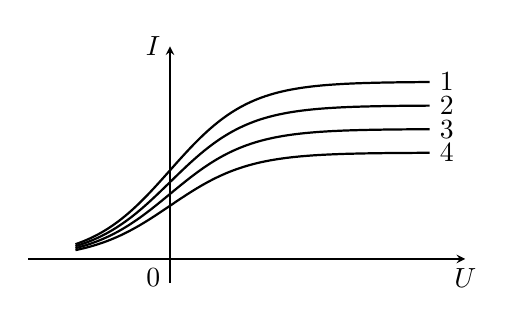
\begin{tikzpicture}[>=stealth, scale=1.5]
  \draw[->] (-1.2,0) -- (2.5,0) node[below] {$U$};
  \draw[->] (0,-0.2) -- (0,1.8) node[left] {$I$};
  \node[below left] at (0,0) {$0$};
  
  \draw[thick, domain=-0.8:2.2, samples=100] plot (\x, {1.5 / (1 + exp(-3*\x))}) node[right] {1};
  \draw[thick, domain=-0.8:2.2, samples=100] plot (\x, {1.3 / (1 + exp(-3*\x))}) node[right] {2};
  \draw[thick, domain=-0.8:2.2, samples=100] plot (\x, {1.1 / (1 + exp(-3*\x))}) node[right] {3};
  \draw[thick, domain=-0.8:2.2, samples=100] plot (\x, {0.9 / (1 + exp(-3*\x))}) node[right] {4};
\end{tikzpicture}
\end{center}

\begin{enumerate}[label=\Alph*)]
\item 4.
\item 3.
\item 2.
\item 1.
\end{enumerate}

\setcounter{enumi}{18}
\item Fotokatod monoxromatik yorug‘lik bilan yoritilganda, undan elektronlar urib chiqariladi. Yorug‘lik chastotasi 2 marta ortganda, chiqayotgan elektronlarning maksimal kinetik energiyasi qanday o‘zgaradi?
\begin{enumerate}[label=\Alph*)]
\item o‘zgarmaydi.
\item 2 martadan ko‘p ortadi.
\item 2 marta ortadi.
\item 2 martadan kam ortadi.
\end{enumerate}

\item Fotokatod monoxromatik yorug‘lik bilan yoritilganda undan elektronlar urib chiqariladi. Yorug‘likning chastotasi 2 marta kamayganda chiqayotgan elektronlarning maksimal kinetik energiyasi qanday o‘zgaradi?
\begin{enumerate}[label=\Alph*)]
\item o‘zgarmaydi.
\item 2 martadan ko‘p kamayadi.
\item 2 marta kamayadi.
\item 2 martadan ko‘p ortadi.
\end{enumerate}

\item Quyidagi hodisalarning qaysilari yorug‘likning to‘lqin nazariyasi asosida tushuntiriladi:
1) difraksiya; 2) interferensiya; 3) fotoeffekt; 4) qutblanish.
\begin{enumerate}[label=\Alph*)]
\item 1, 2 va 4.
\item faqat 1 va 2.
\item faqat 1 va 4.
\item hammasi.
\end{enumerate}

\item Quyidagi hodisalardan qaysilarida oq yorug‘lik monoxromatik nurlarga ajraladi?
1) dispersiya; 2) interferensiya; 3) difraksiya; 4) fotoeffekt; 5) qutblanish.
\begin{enumerate}[label=\Alph*)]
\item 2, 3, 5.
\item 1, 2, 3.
\item 2, 5.
\item 3, 4.
\end{enumerate}

\item Quyidagi hodisalarning qaysilari yorug‘likning kvant nazariyasi asosida tushuntiriladi?
1) difraksiya; 2) interferensiya; 3) fotoeffekt; 4) qutblanish.
\begin{enumerate}[label=\Alph*)]
\item 1 va 3.
\item 2 va 3.
\item 3 va 4.
\item faqat 3.
\end{enumerate}

\end{enumerate}



\begin{table}[!ht]
\centering
\begin{tabular}{|c|c|c|c|c|c|c|c|c|c|c|}
\hline
1d & 2d & 3d & 4b & 5c & 6a & 7b & 8c & 9d & 10b & 11d \\ \hline
12c & 13d & 14d & 15d & 16a & 17d & 18d & 19b & 20b & 21a & 22b \\ \hline
23d & & & & & & & & & & \\ \hline
\end{tabular}
\end{table}